\documentclass[11pt,a4paper]{article}
\usepackage[utf8]{inputenc}
\usepackage[T1]{fontenc}
\usepackage[brazil]{babel}
\usepackage[margin=2cm]{geometry}
\usepackage{amsmath,amssymb}
\usepackage{graphicx}
\usepackage{booktabs}
\usepackage{hyperref}
\usepackage{caption}
\captionsetup{font=small}

\title{Mini-projeto: buscas clássicas e otimização}
\author{Evanielly Correia}
\date{2026}

\begin{document}
\maketitle

\section{Introdução}
Este trabalho resolve o problema de transformar uma sequência de $L$ bits em uma sequência alvo por meio de \emph{bit-flips}, sob duas abordagens: (i) busca clássica no espaço discreto de estados (BFS e busca gulosa) e (ii) otimização contínua por gradiente descendente, com uma penalização que favorece transformações consecutivas. O código está disponível em: \url{https://github.com/evaniellycorreia/mini-projeto-buscas}.

\section{Buscas clássicas}
\subsection{Modelagem}
Cada estado é uma sequência $s\in\{0,1\}^L$. Uma operação inverte um intervalo consecutivo $[i,j]$, com $0\le i\le j<L$, a custo 1 (o flip de um único bit é o caso $i=j$). Cada estado possui, portanto, $L(L+1)/2$ sucessores. Por eficiência, os estados foram representados como inteiros e cada flip foi implementado como uma operação XOR com uma máscara pré-calculada.

\paragraph{Custo ótimo.} Seja $d=s\oplus y$ o vetor de bits errados. Um flip altera no máximo duas fronteiras entre posições certas e erradas; logo, o custo mínimo é igual ao número de blocos consecutivos de bits errados em $d$, e esse valor é atingível invertendo um bloco por vez. Esse resultado foi usado para validar as soluções quando o BFS não era viável (apresentado logo mais).

\subsection{Algoritmos}
\textbf{BFS:} explora os estados por níveis com uma fila FIFO e um dicionário de pais para reconstruir o caminho; como todas as operações têm custo 1, a primeira solução encontrada é ótima.

\textbf{Greedy:} usa a distância de Hamming $h(s)=\sum_k \mathbb{1}(s_k\neq y_k)$ como heurística, pois ela mede diretamente quantas posições ainda diferem do alvo. Para $L$ grande, o melhor sucessor foi obtido sem enumerar os $O(L^2)$ vizinhos: atribuindo ganho $+1$ aos bits errados e $-1$ aos certos, o flip que mais reduz $h$ é o subvetor de soma máxima, encontrado em $O(L)$ pelo algoritmo de Kadane.

\subsection{Resultados}
Para a sequência oficial \texttt{00001001000011001100111} ($L=23$, 5 blocos de bits 1), ambos os algoritmos encontraram soluções válidas de custo 5 (Tabela~\ref{tab:oficial}). O BFS retornou $(4,4),(7,7),(12,13),(16,17),(20,22)$; o Greedy encontrou um caminho distinto e igualmente ótimo, mostrando que a solução ótima não é única.

\begin{table}[h]
\centering
\caption{Sequência oficial.}
\label{tab:oficial}
\begin{tabular}{lrrrr}
\toprule
Algoritmo & Custo & Estados expandidos & Estados visitados & Tempo (s)\\
\midrule
BFS & 5 & 762\,113 & 2\,681\,287 & 22,87\\
Greedy & 5 & 6 & 1\,198 & 0,001\\
\bottomrule
\end{tabular}
\end{table}

\paragraph{Desempenho.} Foram gerados $N=10$ pares aleatórios (semente 42) para cada $L$, e os algoritmos foram executados sobre os mesmos pares. Na comparação direta ($L=2,\dots,256$), o BFS foi limitado a $3\times10^6$ estados visitados. Ele concluiu até $L=16$ (média de $10\,242{,}6$ estados expandidos, contra $4{,}7$ do Greedy) e não concluiu em nenhum par de $L=32$ a $L=256$; em $L=32$, cada tentativa levou de 17 a 37~s até atingir o limite. Esse comportamento evidencia o crescimento exponencial do espaço ($2^L$ estados). O Greedy com fila de prioridade concluiu todos os 10 pares em todos esses tamanhos, com o mesmo custo do BFS sempre que este concluiu, mas seu tempo cresceu até cerca de 7~s por par em $L=256$, devido aos $O(L^2)$ sucessores por estado. Para $L=512,\dots,4096$ foi usada a versão com Kadane. Como a mesma semente gera os mesmos pares, o Greedy obteve o custo ótimo nos 120 pares (Tabela~\ref{tab:greedy}). O custo médio acompanhou $L/4$, valor esperado do número de blocos de bits errados em sequências aleatórias. Em ambas as versões, o Greedy expandiu exatamente custo$\,+1$ estados, ou seja, seguiu direto para o alvo. Nos casos de $L$ muito pequeno, o BFS aparece com menos expansões porque verifica o objetivo ao gerar o estado, enquanto o Greedy o verifica ao retirá-lo da fila.

\begin{table}[h]
\centering
\caption{Greedy (Kadane) versus custo ótimo, médias de 10 pares.}
\label{tab:greedy}
\begin{tabular}{rrrrr}
\toprule
$L$ & Custo Greedy & Custo ótimo & $L/4$ & Tempo (s)\\
\midrule
16 & 3,7 & 3,7 & 4 & 0,00002\\
256 & 64,4 & 64,4 & 64 & 0,0009\\
1024 & 256,1 & 256,1 & 256 & 0,016\\
4096 & 1028,6 & 1028,6 & 1024 & 0,27\\
\bottomrule
\end{tabular}
\end{table}

\begin{figure}[h]
\centering
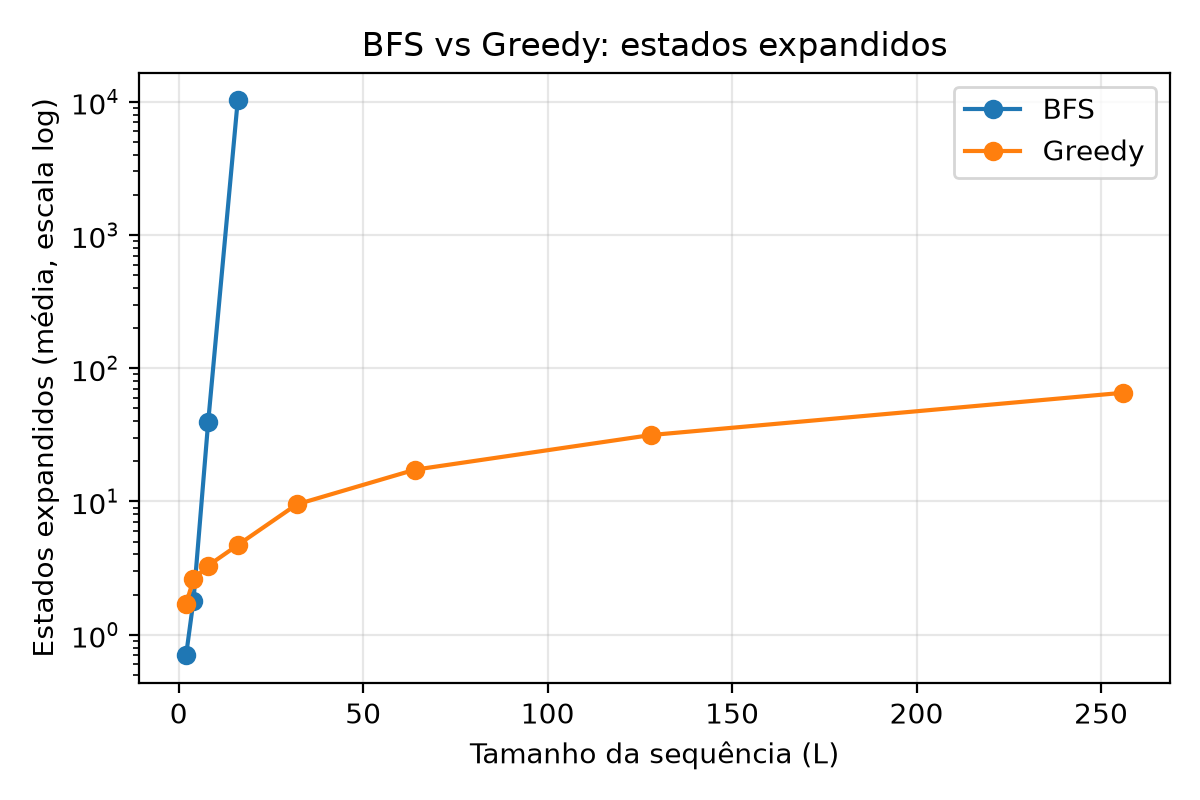
\includegraphics[width=0.32\textwidth]{grafico_expandidos.png}
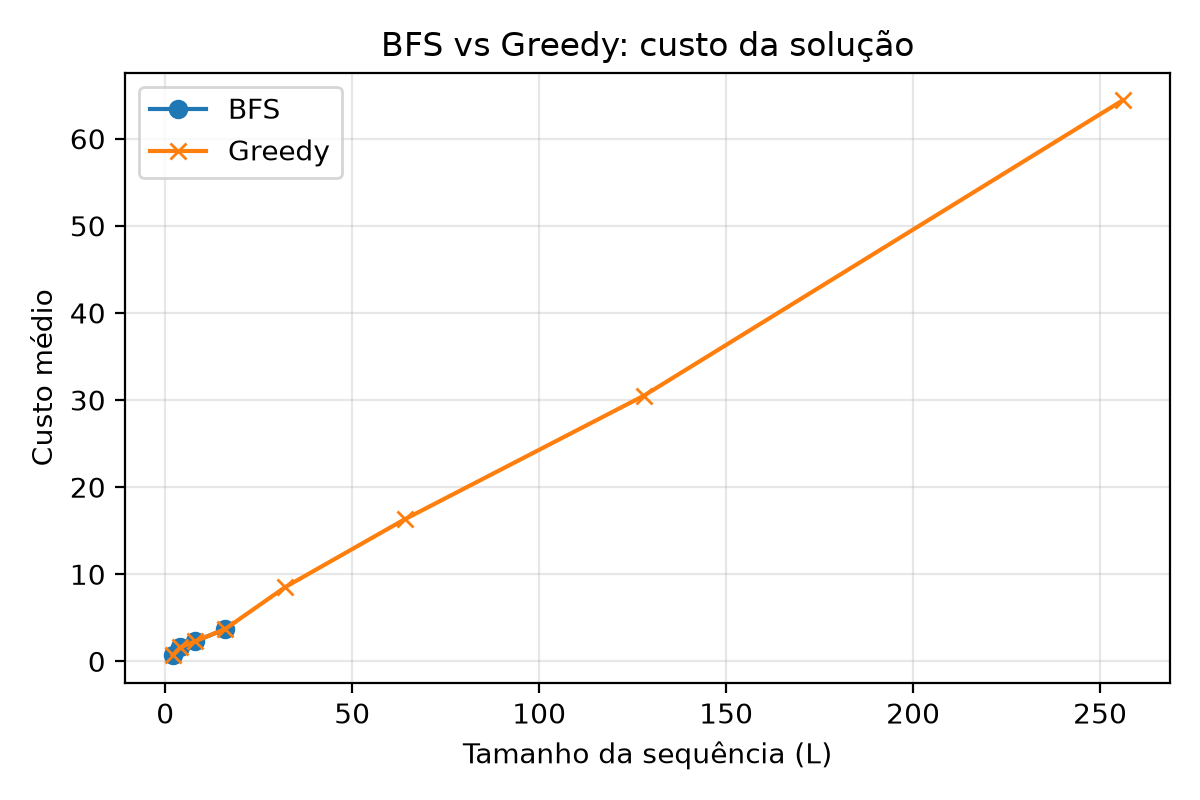
\includegraphics[width=0.32\textwidth]{grafico_custo.png}
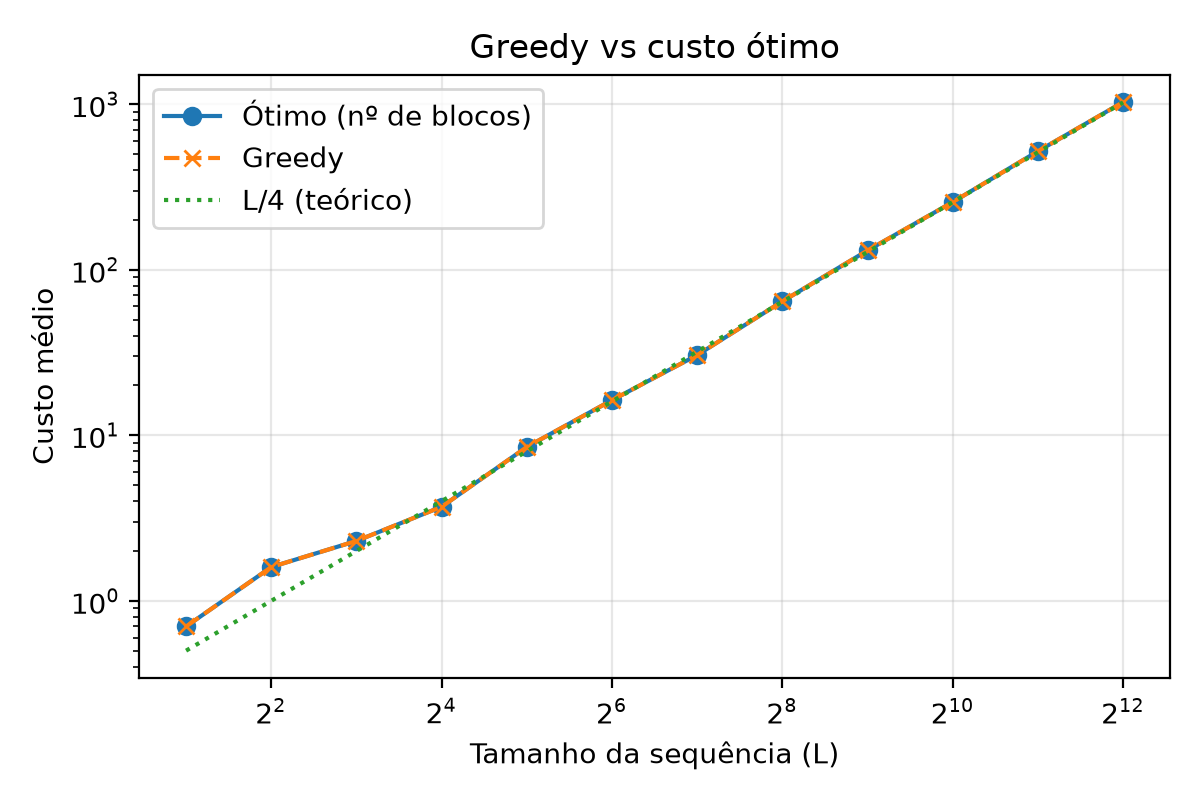
\includegraphics[width=0.32\textwidth]{grafico_custo_grande.png}
\caption{Esquerda: estados expandidos (escala log); o BFS aparece só até $L=16$, pois não concluiu a partir de $L=32$. Centro: custo médio do BFS e do Greedy (curvas sobrepostas onde ambos concluíram). Direita: Greedy, custo ótimo e $L/4$ até $L=4096$.}
\end{figure}

\section{Otimização com gradiente descendente}
\subsection{Função erro}
Cada bit é relaxado para $x_k\in[0,1]$ e o erro é $L(x)=\sum_k (x_k-y_k)^2$. Minimizar $L$ equivale a buscar transformações que levem $x$ ao alvo: $L=0$ se e somente se $x=y$, e, em pontos binários, $L(x)$ coincide com a distância de Hamming. A atualização é
\begin{equation}
x_k \leftarrow x_k-2\eta\,(x_k-y_k),
\end{equation}
e o vetor diferença entre passos consecutivos representa a transformação aplicada.

\subsection{Efeito de $\eta$ - Taxa de Aprendizado}
Para $y_k=0$, obtém-se $x_k\leftarrow(1-2\eta)x_k$. Para $\eta>1/2$, o fator é negativo e o bit troca de sinal: com $x_k=1$ e $\eta=0{,}75$, tem-se $x_k=-0{,}5$, fora de $[0,1]$. Para $\eta\ge1$, $|1-2\eta|\ge1$ e o método não converge: com $\eta=1$, cada bit oscila entre $1$ e $-1$ e o erro permanece 9. Com $\eta=0{,}5$, a convergência ocorre em um passo. As curvas de erro para $\eta=0{,}25$ e $\eta=0{,}75$ coincidem, pois $|1-2\eta|=0{,}5$ nos dois casos; a diferença é que, com $\eta=0{,}75$, o valor oscila em torno do alvo (Figura~\ref{fig:eta}).

\begin{figure}[h]
\centering
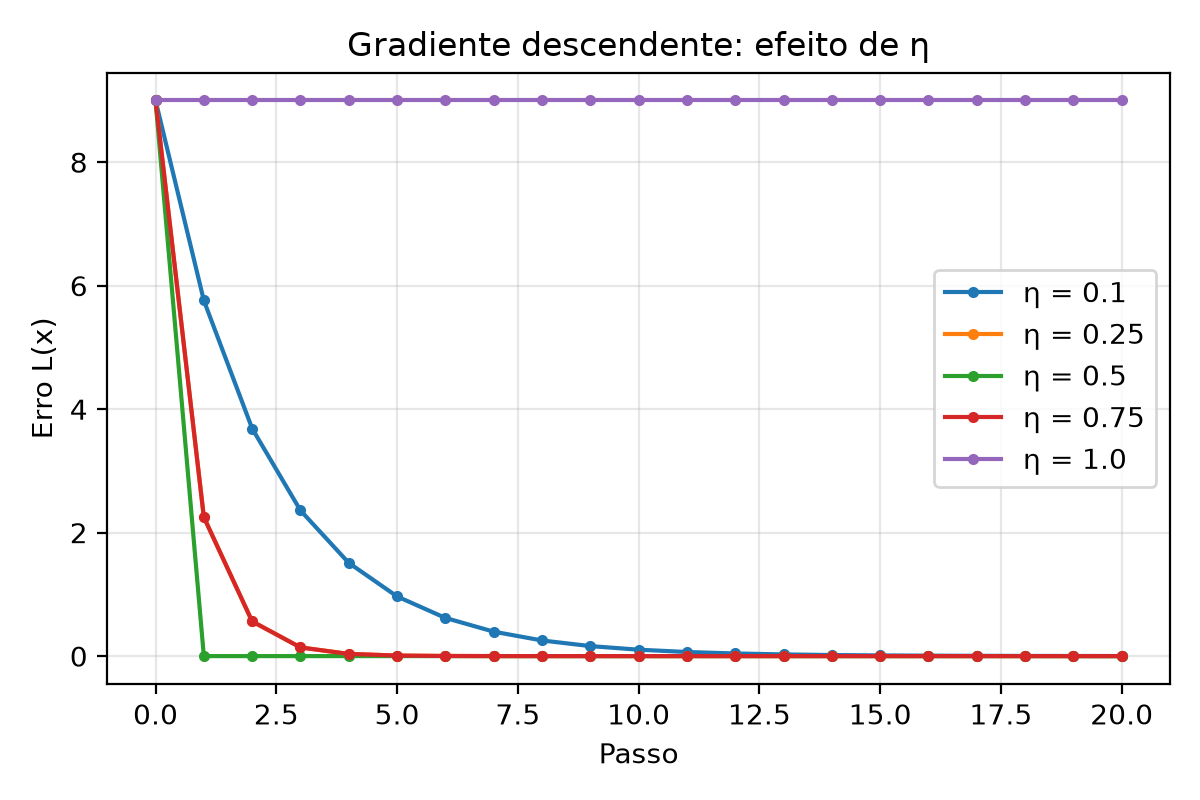
\includegraphics[width=0.45\textwidth]{grafico_eta.png}
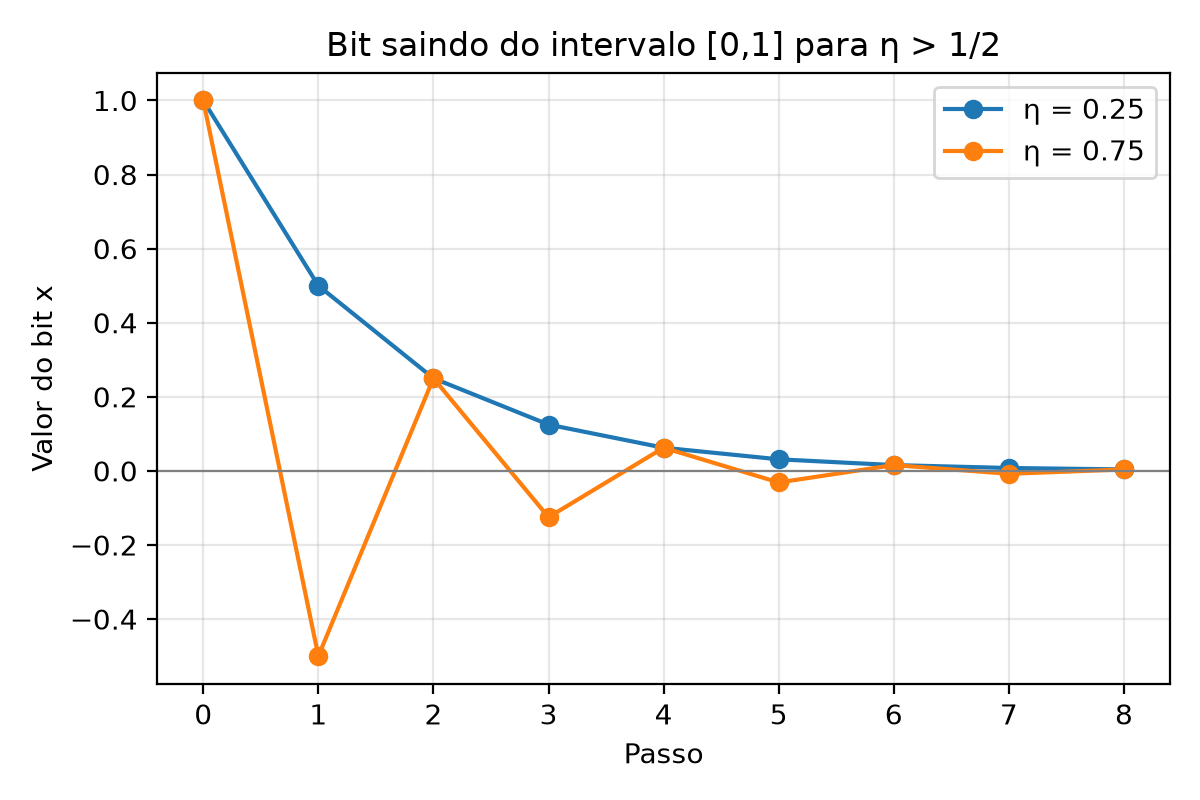
\includegraphics[width=0.45\textwidth]{grafico_bit_negativo.png}
\caption{Esquerda: erro $L(x)$ por passo para diferentes $\eta$. Direita: bit com $x=1$, $y=0$; para $\eta=0{,}75$ o valor atinge $-0{,}5$.}
\label{fig:eta}
\end{figure}

\subsection{Custo de transformações não consecutivas}
Definiu-se a intensidade da mudança em cada posição como uma função suave do gradiente:
\begin{equation}
g_i=\frac{\partial L}{\partial x_i}=2(x_i-y_i),\qquad z_i=\sqrt{g_i^2+\varepsilon},
\end{equation}
e o custo
\begin{equation}
C(z)=\sum_{i=1}^{L-1}(z_{i+1}-z_i)^2,
\end{equation}
que é pequeno quando posições vizinhas mudam com intensidades semelhantes (blocos) e penaliza mudanças isoladas. Para $J(x)=L(x)+\lambda C(z)$, a regra da cadeia fornece
\begin{equation}
\frac{\partial J}{\partial x_i}=2(x_i-y_i)+\lambda\big[2(z_i-z_{i-1})-2(z_{i+1}-z_i)\big]\frac{2g_i}{z_i}.
\end{equation}
O termo entre colchetes depende de $z_{i-1}$ e $z_{i+1}$; portanto, a variação de $x_i$ recebe contribuições do custo das transformações adjacentes. O gradiente analítico foi conferido por diferenças finitas (diferença máxima de $2{,}93\times10^{-8}$).

\subsection{Resultados para $\lambda$ - Priorização do passo}
A minimização usou $\eta=0{,}05$ e 300 passos. Todos os valores convergiram para o alvo, então o efeito de $\lambda$ aparece no caminho (Tabela~\ref{tab:lambda}): quanto maior $\lambda$, menor o custo $C$ ao longo das transformações, ou seja, mudanças mais uniformes entre vizinhos. Nesta formulação, $\lambda$ maior também acelerou a convergência, pois a penalização aumenta o passo efetivo; valores muito altos podem, por isso, causar instabilidade. A Figura~\ref{fig:lambda} mostra que, com $\lambda$ maior, os blocos $(12,13)$ e $(16,17)$ e os bits isolados avançam de forma mais rápida e uniforme dentro de cada bloco. Por outro lado, no bloco $(20,22)$ as extremidades passam a receber intensidades diferentes, porque a penalização também considera as fronteiras com os vizinhos já corretos.

\begin{table}[h]
\centering
\caption{Efeito de $\lambda$ na sequência oficial.}
\label{tab:lambda}
\begin{tabular}{rrrr}
\toprule
$\lambda$ & Passos até $L<10^{-6}$ & $C$ médio no caminho & $C$ no passo 10\\
\midrule
0 & 76 & 0,6283 & 4,3642\\
0,01 & 74 & 0,5961 & 3,8417\\
0,1 & 66 & 0,4202 & 1,3451\\
1 & 40 & 0,1532 & 0,0417\\
\bottomrule
\end{tabular}
\end{table}

\begin{figure}[h]
\centering
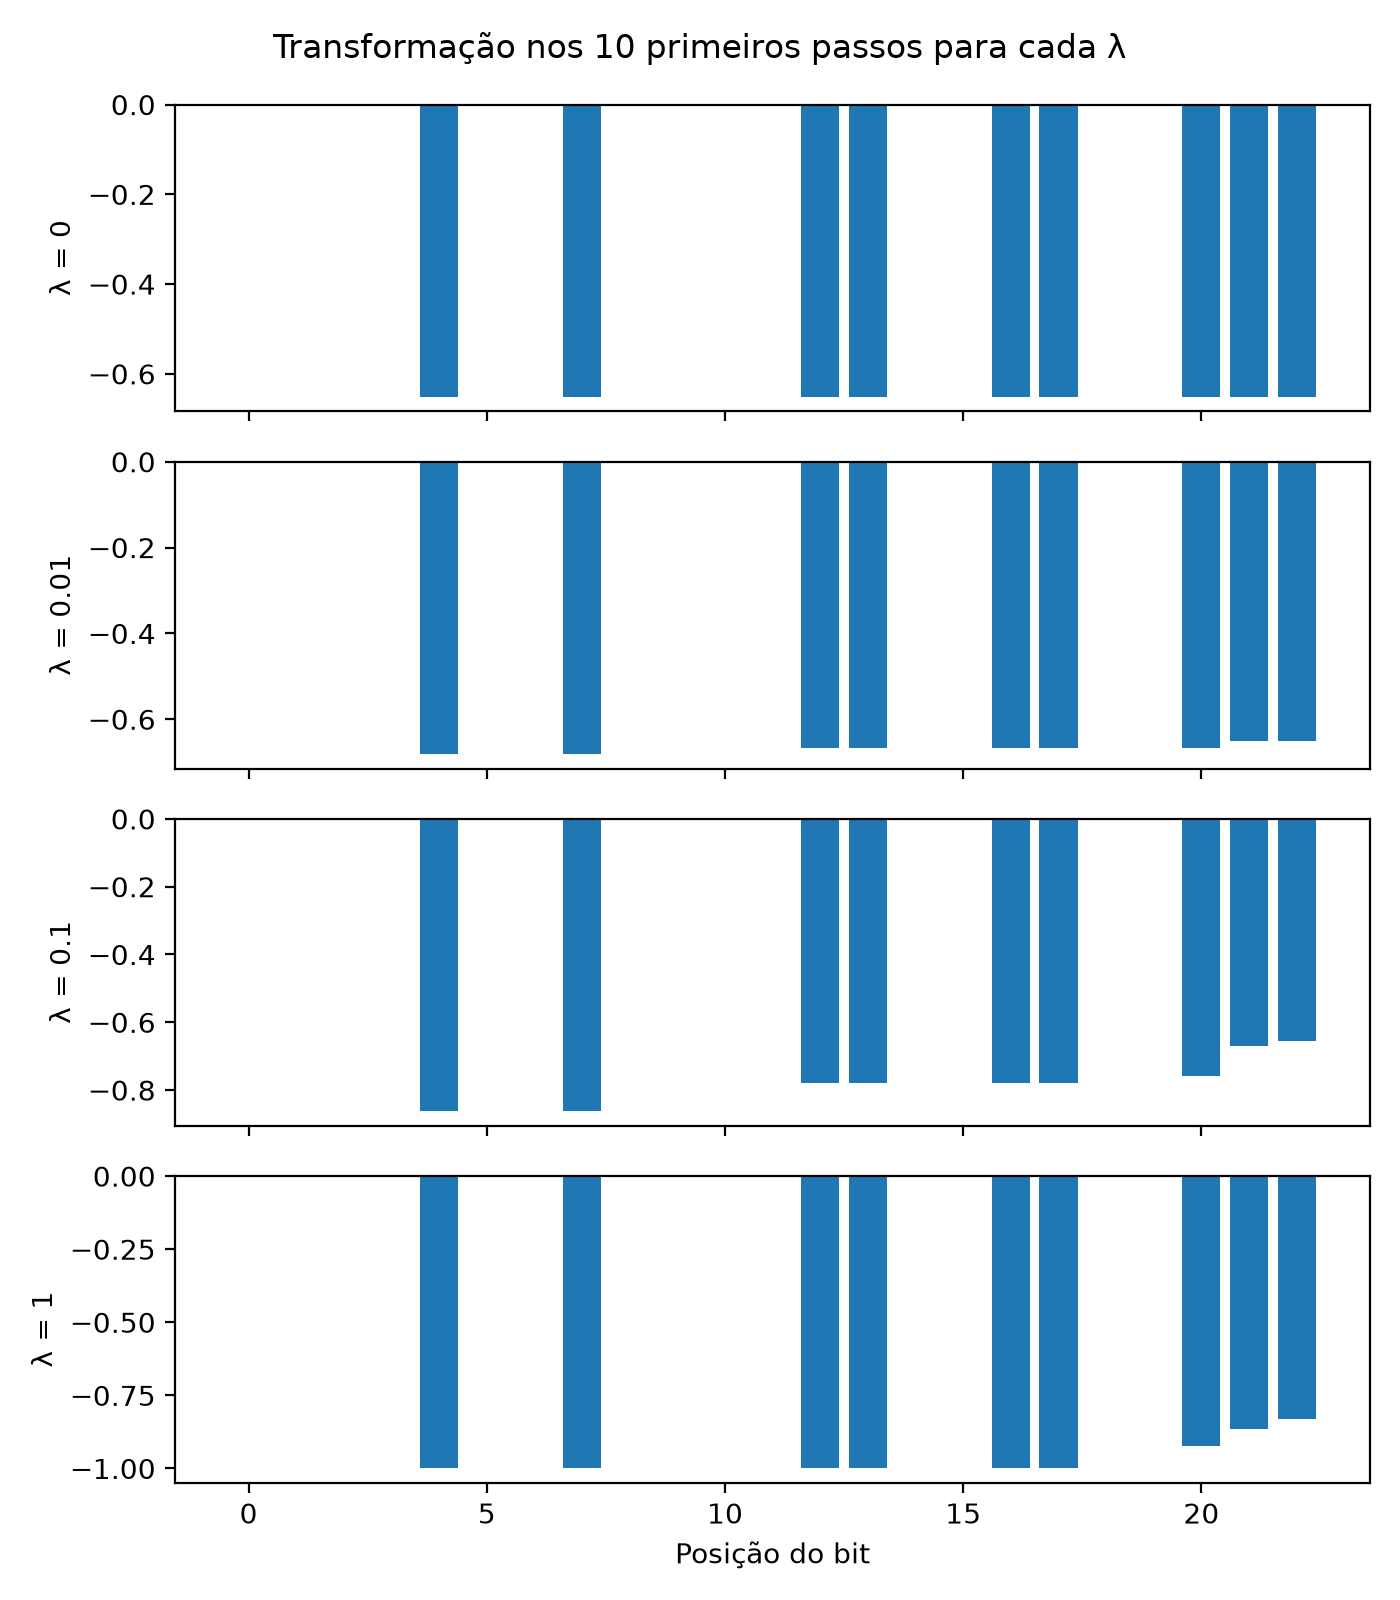
\includegraphics[width=0.55\textwidth]{grafico_lambda.png}
\caption{Transformação acumulada nos 10 primeiros passos, por posição, para cada $\lambda$.}
\label{fig:lambda}
\end{figure}

\section{Conclusão}
O BFS garante a solução ótima, mas tornou-se inviável a partir de $L=32$ devido ao crescimento exponencial do espaço de estados. O Greedy com distância de Hamming encontrou o custo ótimo em todos os casos testados e, com o algoritmo de Kadane, escalou até $L=4096$. Na abordagem contínua, $\eta$ controla estabilidade e validade dos valores ($\eta>1/2$ produz valores fora de $[0,1]$), enquanto $\lambda$ controla o compromisso entre aproximar o alvo e realizar mudanças consecutivas.

\end{document}
